\chapter{Resultados y análisis}

Como se mencionó anteriormente, se implementaron tres algoritmos diferentes (RA1, LRDEA y GA-Nuggets) y se realizó la experimentación utilizando los datos obtenidos de tres autómatas celulares diferentes (AC Brain, AC Byl, AC Evoloops y AC Mite). Para cada uno de los experimentos realizados con los autómatas celulares, se utilizaron los siguientes parámetros:
\\
\begin{itemize}
	\item \textbf{Vecindario:} de tipo Moore con 8 vecinos.
	\item \textbf{Parámetros de GA-Nuggets:}
	\begin{itemize}
		\item $w1=1$ 
		\item $w2=2$ 
		\item $\beta=2$ 
		\item $pMutacion=0.05$
		\item $noHijos=2$ 
		\item $poblacion=100$ 
		\item $noIteraciones=100$
		\item $maximoAntecedente=50$
		\item $minimoAntecedente=3$
	\end{itemize}
	\item \textbf{Parámetros de LRDEA:}
	\begin{itemize}
		\item $noHijos=2$
		\item $poblacion=100$
		\item $pMutacion=0.05$
		\item $noIteraciones=100$
	\end{itemize}
	\item \textbf{Parámetros de RA1:}
	\begin{itemize}
		\item $l=5$
	\end{itemize}
\end{itemize}

El algoritmo RA1, al contrario del algoritmo GA-Nuggets y el algoritmo LRDEA, es un algoritmo cuyo funcionamiento depende solamente de una variable aleatoria. Esto se debe a que, como es un algoritmo \emph{avaro}, existe la posibilidad de que se quede estancado en un óptimo local; para evitar esto, es necesaria la mencionada variable aleatoria.
\\

Finalmente, se puede notar en los parámetros que se enlistan arriba, que se requieren configurar menos parámetros para los algoritmos RA1 y LRDEA en comparación con el algoritmo GA-Nuggets.


\section{Brain}
En las figuras \ref{fig:ra1brain}, \ref{fig:lrdeabrain} y \ref{fig:ganuggetsabrain} se muestran los resultados de exactitud de la implementación de cada uno de los tres algoritmos para los datos obtenidos del AC Brain.
\\

Estos resultados de exactitud o \emph{accuracy} se muestran a partir del paso de simulación o \emph{Simultion step} número 160, debido a que los estados previos (1-159) se utilizan para el proceso de entrenamiento, y el estado 160 se utiliza para calcular el error de aprendizaje, exactitud de entrenamiento o \emph{train accuracy}.
\\

El otro dato que se visualiza en las gráficas, denominado error de generalización, exactitud de prueba o \emph{test accuracy}, se calcula con un estado que no se le ha mostrado al algoritmo en el entrenamiento, en este caso, se calcula la exactitud de prueba con el estado siguiente (161).
\\

De manera general, para calcular la exactitud de entrenamiento del estado \textit{n}, se toma como conjunto de entrenamiento los \textit{n-1} estados previos y finalmente se compara el estado \textit{n} con el estado \textit{n} que se predijo. Mientras que para calcular la exactitud de prueba del estado \textit{n}, se toma el estado \textit{n+1} (no mostrado previamente).
\\

Según el diagrama de la figura \ref{fig:walkforward}, el conjunto de entrenamiento (en azul) serían los estados previos a \textit{n}, el dato para calcular la exactitud de entrenamiento \textit{n} sería el amarillo y el dato \textit{n+1}, utilizado para calcular la exactitud de prueba, sería el dato rojo.
\\

Como se puede observar en la figura \ref{fig:ra1brain}, el algoritmo RA1 tuvo un desempeño superior a los otros algoritmos con un promedio de exactitud de 89\% dentro del conjunto de entrenamiento y de 85\% fuera del conjunto de entrenamiento, a comparación del algoritmo LRDEA (figura \ref{fig:lrdeabrain}) que obtuvo un promedio de 88\% y 81\% respectivamente, y el algoritmo GA-Nuggets con 88\% y 79\% (figura \ref{fig:ganuggetsabrain}).

	\begin{figure}[H]
		\centering
		\includegraphics[width=\linewidth]{fig/ra1_0}
		\caption{Exactitud de el algoritmo RA1 sobre el conjunto de datos del AC Brain.}
		\label{fig:ra1brain}
	\end{figure}

	\begin{figure}[H]
		\centering
		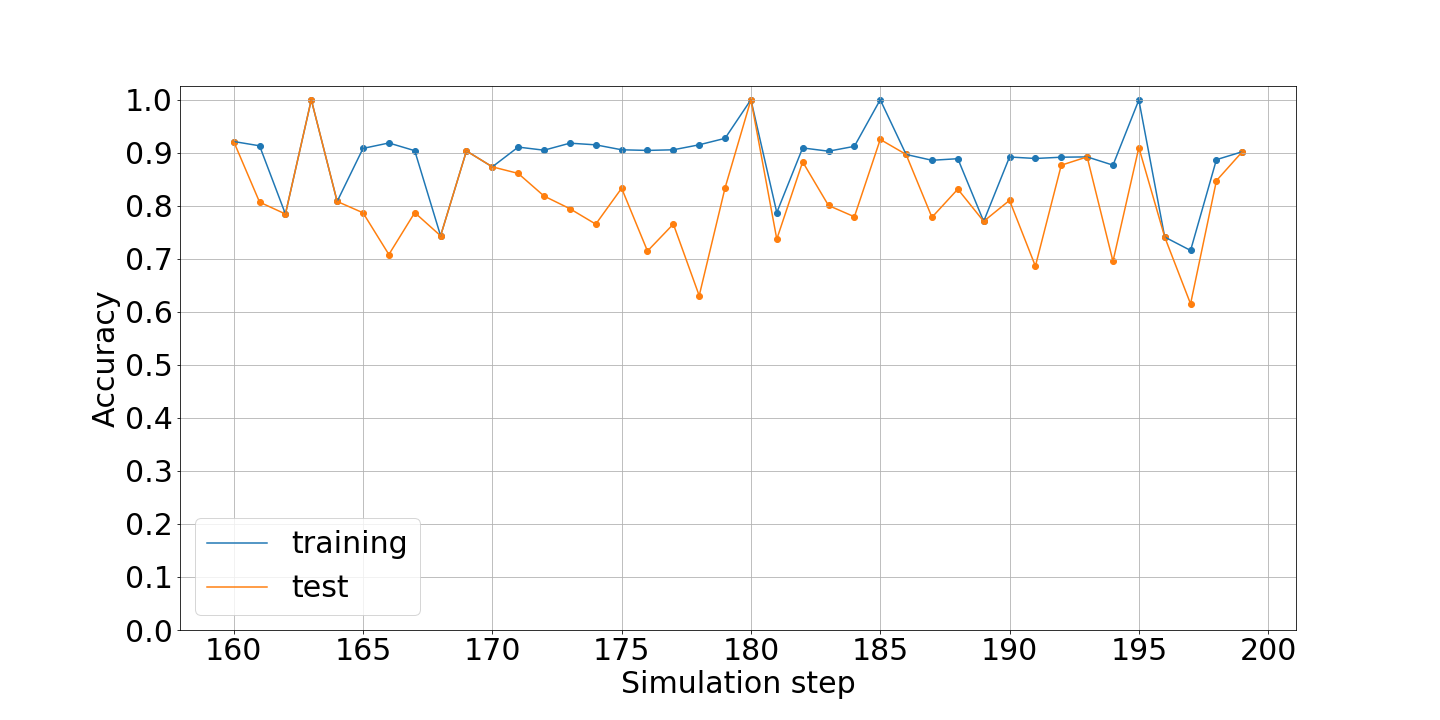
\includegraphics[width=\linewidth]{fig/LRDEA_1}
		\caption{Exactitud de el algoritmo LRDEA sobre el conjunto de datos del AC Brain.}
		\label{fig:lrdeabrain}
	\end{figure}

	\begin{figure}[H]
		\centering
		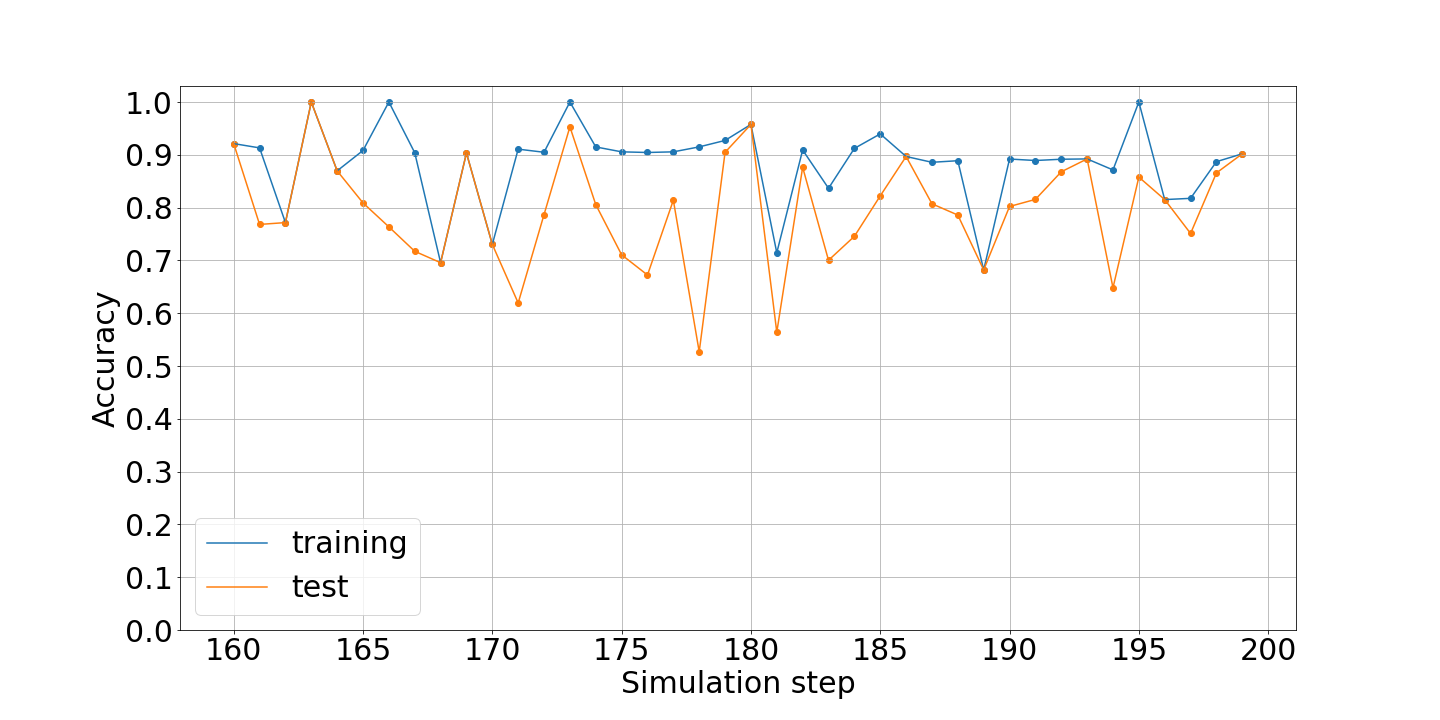
\includegraphics[width=\linewidth]{fig/GA-nuggets_2}
		\caption{Exactitud de el algoritmo GA-Nuggets sobre el conjunto de datos del AC Brain.}
		\label{fig:ganuggetsabrain}
	\end{figure}

\section{Byl}
De manera similar a la presentación de los resultados anteriores, en las figuras \ref{fig:ra1byl}, \ref{fig:lrdeabyl} y \ref{fig:ganuggetsabyl} se muestran los resultados de exactitud de los tres algoritmos implementados en los datos del AC Byl.
\\

Como se logra apreciar en las figuras a continuación, en ciertos pasos de la simulación se logró obtener una exactitud del 100\%, esto es debido a que ciertos estados tienen un comportamiento más trivial que los otros, lo que resulta más fácil de aprender para los algoritmos.
\\

De la misma forma que los resultados para los datos del AC Brain, el algoritmo que obtuvo mejor valor de exactitud fue el RA1 con un promedio de 90\% en el conjunto de entrenamiento y un 85\% fuera del conjunto de entrenamiento.
\\

A su vez, el algoritmo LRDEA obtuvo un promedio de 91\% y 84\% , lo que nos indica que el algoritmo tiene más variación con respecto al RA1. Por último, el algoritmo GA-Nuggets obtuvo 89\% y 77\% con mayor variación y menor valor de exactitud con respecto a los otros dos algoritmos.
\begin{figure}[H]
	\centering
	\includegraphics[width=\linewidth]{fig/ra1_3}
	\caption{Exactitud de el algoritmo RA1 sobre el conjunto de datos del AC Byl.}
	\label{fig:ra1byl}
\end{figure}

Es interesante notar cómo en la figura \ref{fig:lrdeabyl} y la figura \ref{fig:ganuggetsabyl} se ve un comportamiento similar, a comparación con la figura \ref{fig:ra1byl}. Esto puede deberse a las dinámicas que rigen a los algoritmos genéticos, se podría esperar que el algoritmo RA1 sea menos propenso a variaciones porque depende en menor medida de la probabilidad.
\begin{figure}[H]
	\centering
	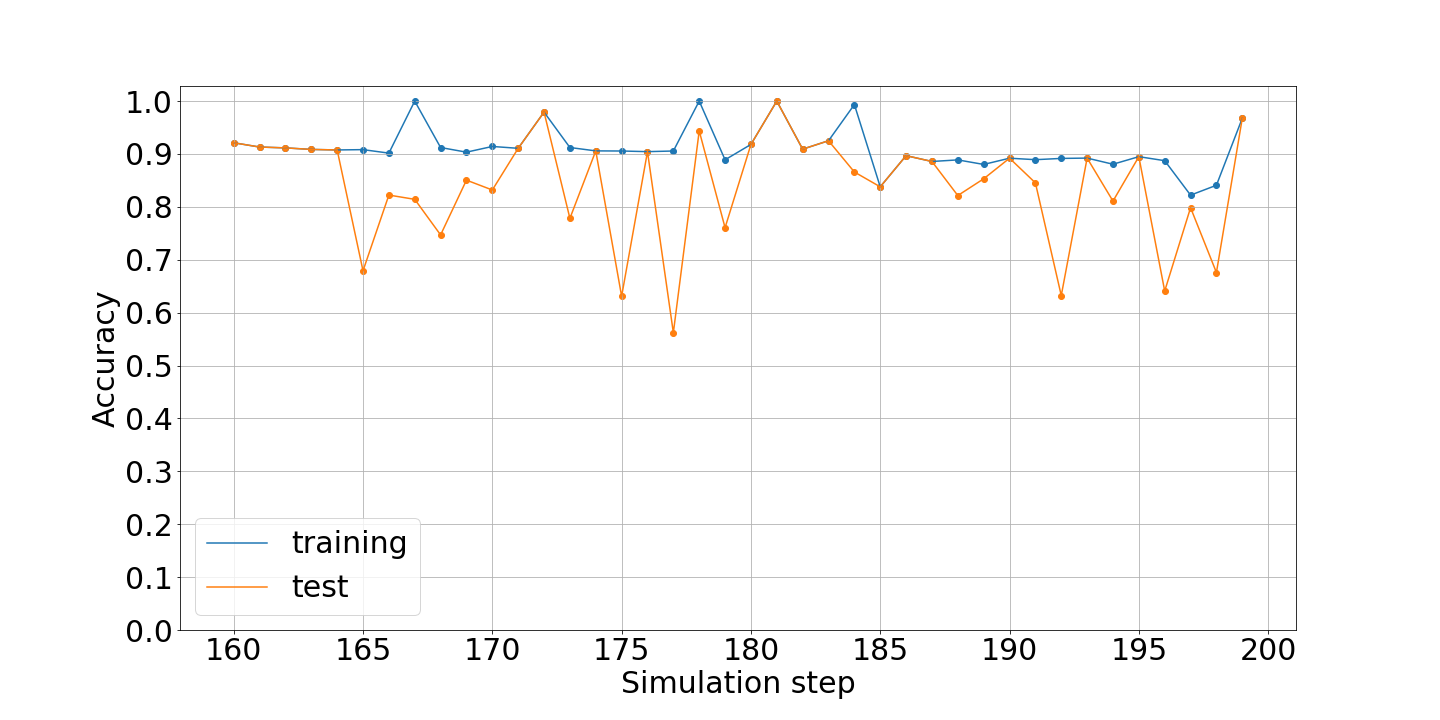
\includegraphics[width=\linewidth]{fig/LRDEA_4}
	\caption{Exactitud de el algoritmo LRDEA sobre el conjunto de datos del AC Byl.}
	\label{fig:lrdeabyl}
\end{figure}

\begin{figure}[H]
	\centering
	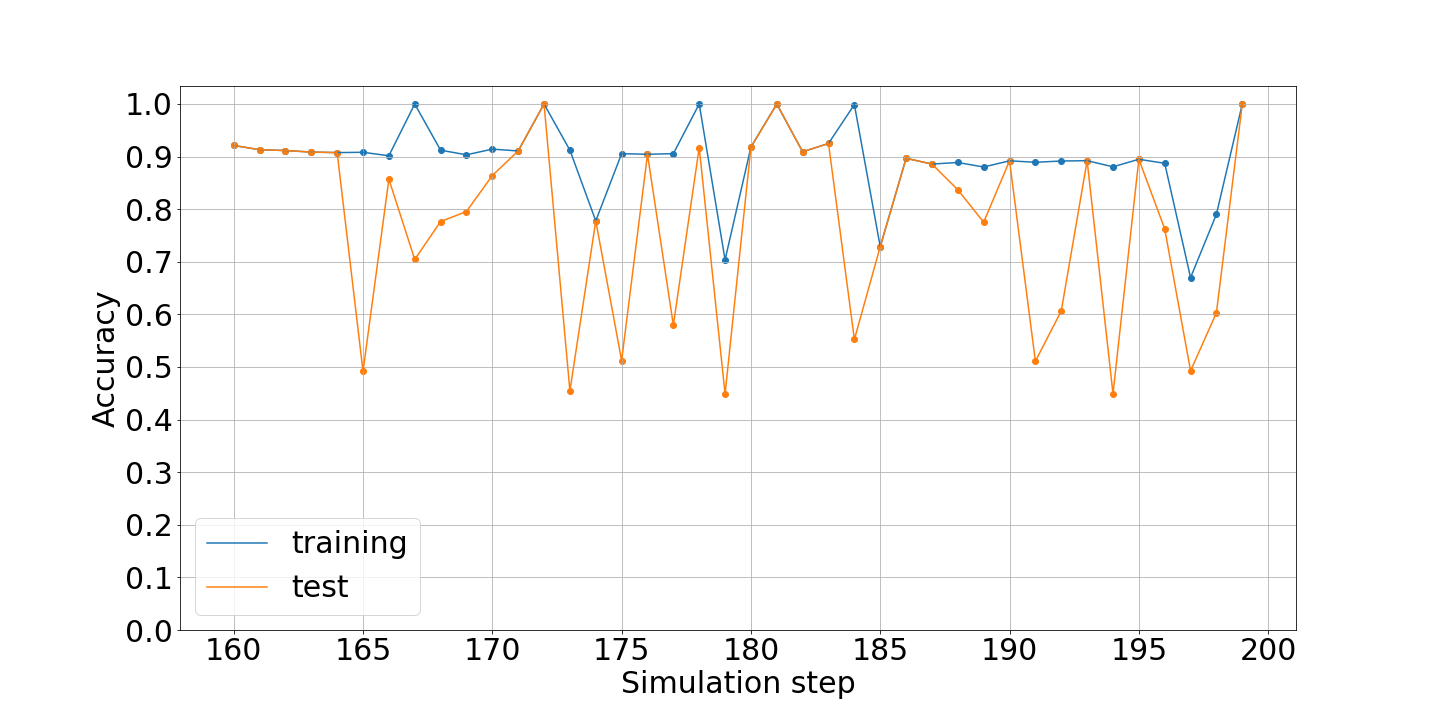
\includegraphics[width=\linewidth]{fig/GA-nuggets_5}
	\caption{Exactitud de el algoritmo GA-Nuggets sobre el conjunto de datos del AC Byl.}
	\label{fig:ganuggetsabyl}
\end{figure}

\section{Evoloops}
En este experimento, al igual que con el AC Byl, el algoritmo RA1 obtuvo un desempeño superior al algoritmo LRDEA Y GA-nuggets, con un promedio de 90\% de exactitud dentro del entrenamiento y 86\% fuera de entrenamiento. En segundo lugar, se encuentra el algoritmo LRDEA con 89\% y 82\% y, por último, el algoritmo GA-Nuggets con 88\% y 78\%.
\begin{figure}[H]
	\centering
	\includegraphics[width=\linewidth]{fig/ra1_6}
	\caption{Exactitud de el algoritmo RA1 sobre el conjunto de datos del AC Evoloops.}
	\label{fig:ra1evoloops}
\end{figure}
\begin{figure}[H]
	\centering
	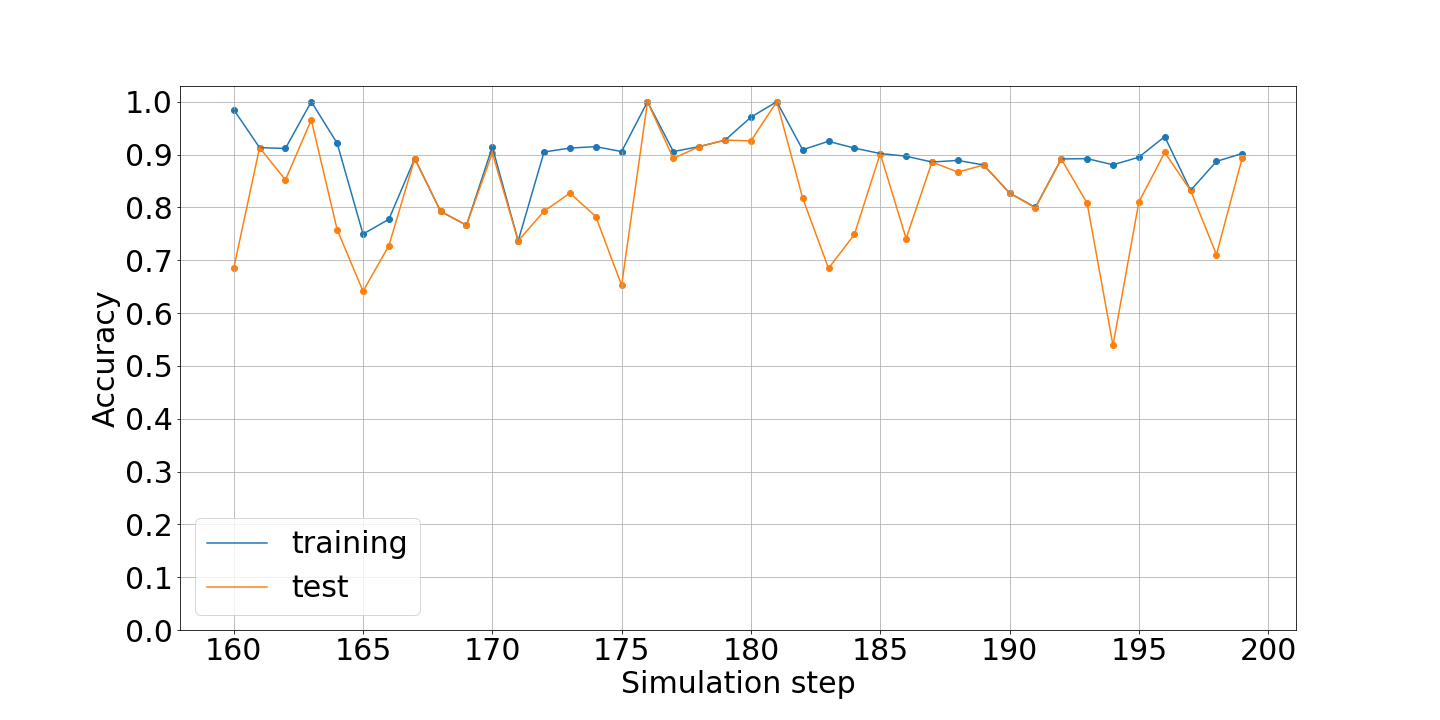
\includegraphics[width=\linewidth]{fig/LRDEA_7}
	\caption{Exactitud de el algoritmo LRDEA sobre el conjunto de datos del AC Evoloops.}
	\label{fig:lrdeaevoloops}
\end{figure}

En la siguiente gráfica se puede observar cómo el GA-Nuggets puede tener mucha variación en su exactitud, en comparación a los otros dos algoritmos.

\begin{figure}[H]
	\centering
	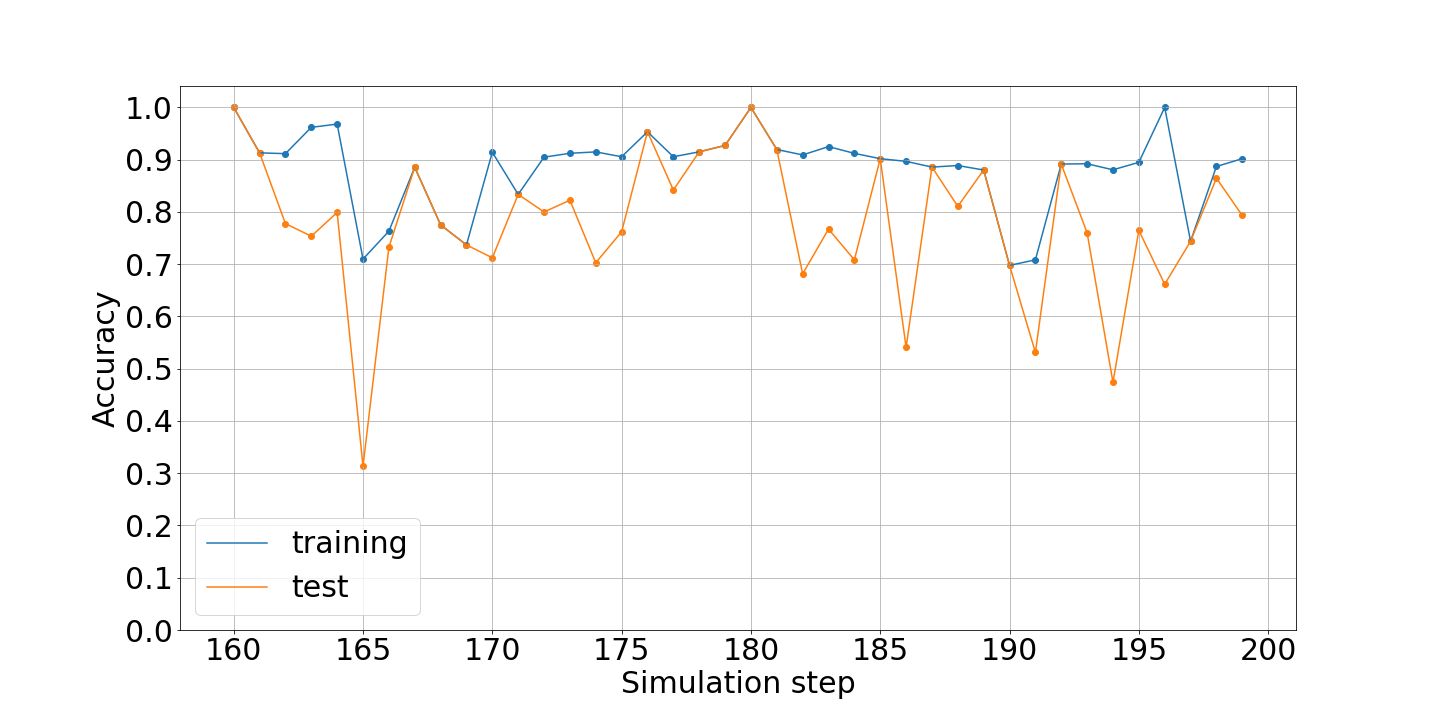
\includegraphics[width=\linewidth]{fig/GA-nuggets_8}
	\caption{Exactitud de el algoritmo GA-Nuggets sobre el conjunto de datos del AC Evoloops.}
	\label{fig:ganuggetsevoloops}
\end{figure}

\section{Mite}
Este experimento fue en el cual se obtuvieron los resultados más bajos, sin embargo, aun así podemos ver que la propuesta (LRDEA) sigue siendo capaz de mantener resultados en promedio superiores a los resultados del algoritmo GA-Nuggets.

Los promedios de exactitud dentro y fuera de entrenamiento para los datos del AC Mite, son los siguientes: RA1 con 89\% y 84\%, LRDEA con 89\% y 81\%, y por último GA-Nuggets con 88\% y 75\%, respectivamente.

\begin{figure}[H]
	\centering
	\includegraphics[width=\linewidth]{fig/ra1_9}
	\caption{Exactitud de el algoritmo RA1 sobre el conjunto de datos del AC Mite.}
	\label{fig:ra1mite}
\end{figure}
\begin{figure}[H]
	\centering
	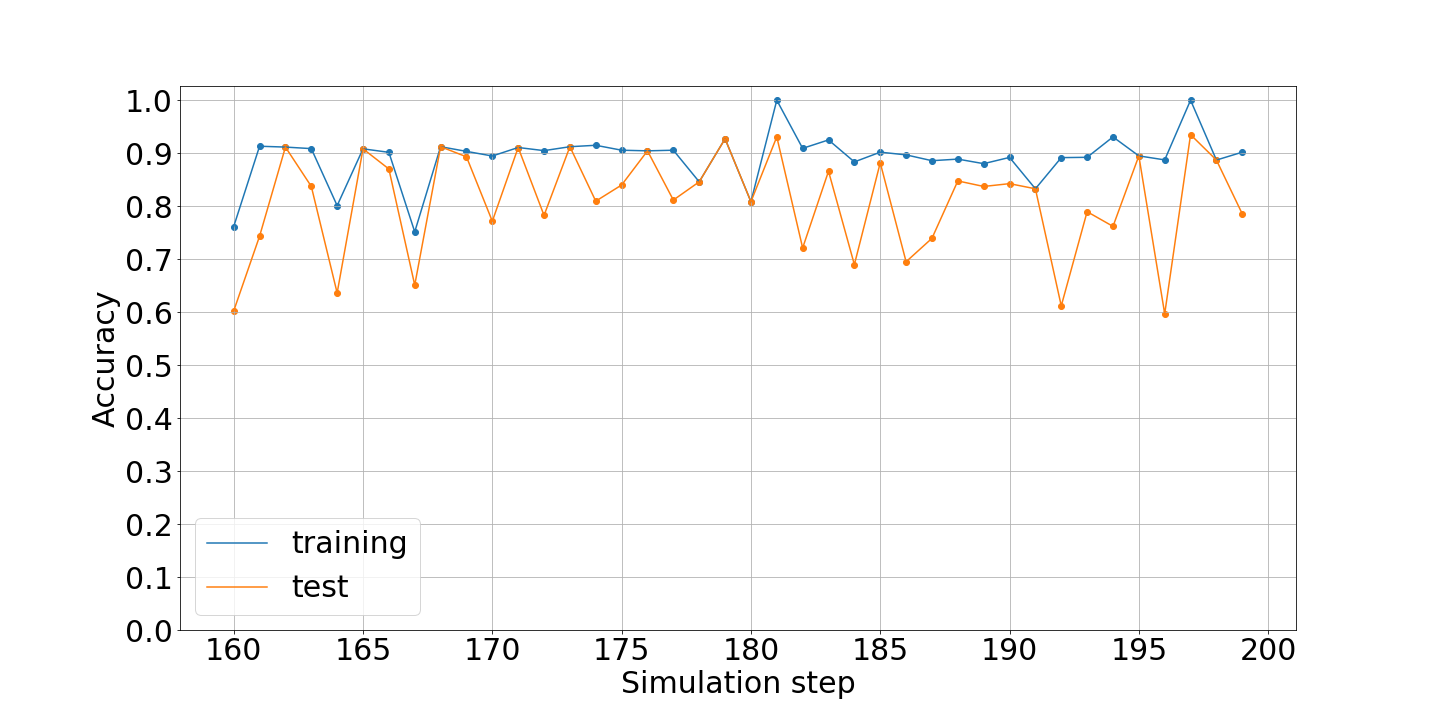
\includegraphics[width=\linewidth]{fig/LRDEA_10}
	\caption{Exactitud de el algoritmo LRDEA sobre el conjunto de datos del AC Mite.}
	\label{fig:lrdeamite}
\end{figure}

\begin{figure}[H]
	\centering
	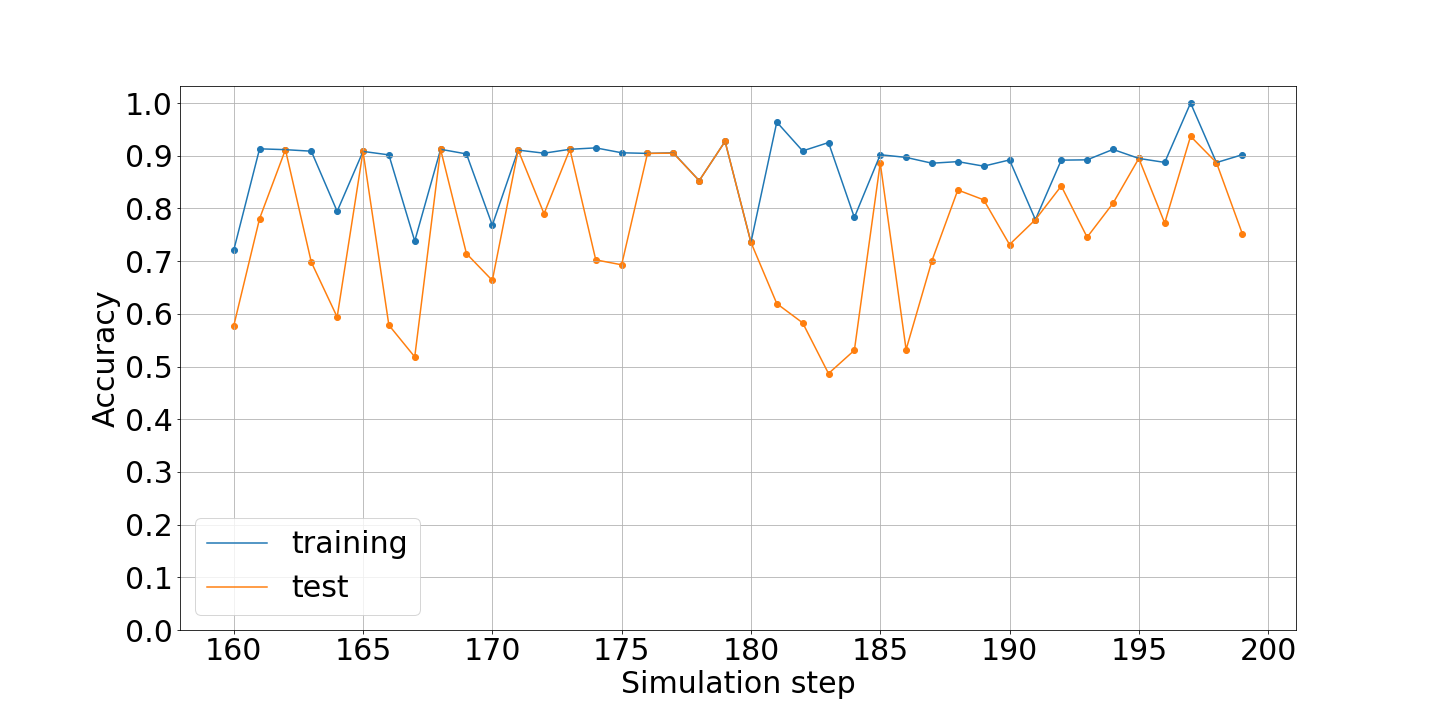
\includegraphics[width=\linewidth]{fig/GA-nuggets_11}
	\caption{Exactitud de el algoritmo GA-Nuggets sobre el conjunto de datos del AC Mite.}
	\label{fig:ganuggetsmite}
\end{figure}



En la siguiente tabla se resumen los resultados obtenido por los algoritmos en cada uno de los experimentos.

%\begin{table}[H]
%	\begin{center}
%		\renewcommand{\arraystretch}{1.2}
%		\resizebox{\textwidth}{!}{%

\begin{table}[H]
	\begin{center}
		\resizebox{\textwidth}{!}{%
		\begin{tabular}{| c |c c| c c| c c |}
			\hline
			\multirow{2}{0.1\linewidth}{}&\multicolumn{2}{|c|}{\textbf{RA1}}&\multicolumn{2}{|c|}{\textbf{LRDEA}}&\multicolumn{2}{|c|}{\textbf{GA-Nuggets}}\\
			\cline{2-7}
			&\textbf{\scriptsize Entrenamiento}&\textbf{\scriptsize Generalización}&\textbf{\scriptsize Entrenamiento}&\textbf{\scriptsize Generalización}&\textbf{\scriptsize Entrenamiento}&\textbf{\scriptsize Generalización}\\
			\hline
			Brain&0.89&0.85&0.88&0.81&0.88&0.79\\
			\hline
			Byl&0.90&0.85&0.91&0.84&0.89&0.77\\
			\hline
			Evoloops&0.90&0.86&0.89&0.82&0.88&0.78\\
			\hline
			Mite&0.89&0.84&0.89&0.81&0.88&0.75\\
			\hline
		\end{tabular}
	}
		\caption{Resultados de la evaluación de los algoritmos. }
		\label{fig:resultsfinal}
	\end{center}
\end{table}
